\subsection{Poruszanie postaci wrogów}\label{subsec:poruszanie_wrogow}

Poruszanie wrogów odbywa się autonomicznie. Droga jest wyliczana, a koordynacje postaci zmieniane są zgodnie z wyliczoną drogą, dzięki czemu postacie wroga przemieszczają się płynnie w kierunku zdefiniowanego celu.

Unity posiada mechanizm wyznaczania dróg na mapie terenu (więcej informacji na ten temat w dziale~\ref{subsec:budowa_terenu} na stronie \pageref{subsec:budowa_terenu}). Aby móc z niego skorzystać, dodaliśmy do postaci wroga agenta nawigacji \name{NavAgent}. Jest to komponent zajmujący się obliczeniami drogi i zarządzaniem przemieszczeniem i obrotem postaci w czasie. Podstawowym parametrem jest 3-wymiarowy wektór określający docelową pozycję, silnik gry zajmuje się wyliczeniem trasy prowadzącej do punktu.

Mechanika wrogów polega na wyszukiwaniu najbliżej znajdującej się postaci gracza, a następnie ustaleniu jej jako cel podążania wroga. W momencie, gry wróg znajduje się odpowiednio blisko, rozpoczyna atak.
\\
\begin{lstlisting}[caption={Algorytm zwracający wskaźnik do obiektu znajdującego się najbliżej, przy określonym maksymalnym promieniu poszukiwań}]
GameObject findNearestPlayer(float maxDistance)
{
    GameObject[] players = GameObject.FindGameObjectsWithTag("Player");
    GameObject nearestPlayer = null;
    float distance = maxDistance;
    foreach (GameObject player in players)
    {
        float distanceFromEnemy = Vector3.Distance(player.transform.position, transform.position);
        if (distanceFromEnemy < distance)
        {
            distance = distanceFromEnemy;
            nearestPlayer = player;
        }
    }
    return nearestPlayer;
}
\end{lstlisting}

\begin{figure}[H]
\center
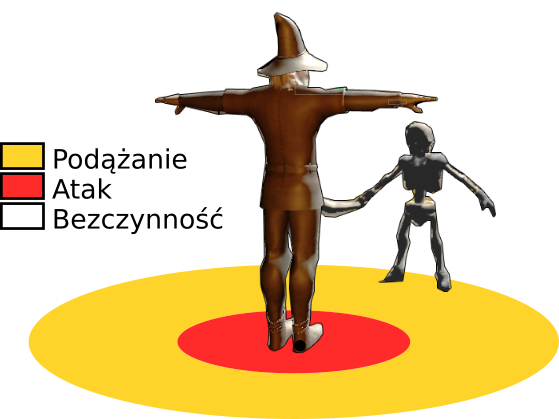
\includegraphics[width=\textwidth]{poruszanie_wrogow_1.png}
\caption{Obszary interakcji postaci wroga}
\end{figure}

W przypadku, gdy wróg ``widzi,, postać gracza, jest w jego stronę stale odwrócony. Służy do tego algorytm, który najpierw wylicza kierunek w postaci wektora wartości w skalu 0.0f..1.0f w przestrzeni 3D, a następnie zamienia wektor na kąt, do którego stopniowo dąży. Daje to efekt płynnego obracania postaci wroga z możliwością dostosowania prędkości obrotu, aby ruchy wyglądały naturalnie, a wróg dawał możliwość np. zajścia go od tyłu.
\\
\begin{lstlisting}[caption={Algorytm zwracający wskaźnik do obiektu znajdującego się najbliżej, przy określonym maksymalnym promieniu poszukiwań}]
private void rotateTowards(Transform target)
{
    Vector3 direction = (target.position - transform.position).normalized;
    Quaternion lookRotation = Quaternion.LookRotation(direction);
    transform.rotation = Quaternion.Slerp(transform.rotation, lookRotation, Time.deltaTime * 5);
}
\end{lstlisting}